\chapter{Data and MC samples}
\label{ch:ana-intro}

\section{Data samples}
The pp collisions at a centre-of-mass
energy of 13~TeV recorded between 2015 and 2017 are used in this search, while the Good-Run-Lists are showed below:
\begin{itemize}
        \scriptsize
\item \texttt{data15\_13TeV.periodAllYear\_DetStatus-v89-pro21-02\_Unknown\_PHYS\_StandardGRL\_All\_Good\_25ns.xml}
\item \texttt{data16\_13TeV.periodAllYear\_DetStatus-v89-pro21-01\_DQDefects-00-02-04\_PHYS\_StandardGRL\_All\_Good\_25ns.xml}
\item \texttt{data17\_13TeV.periodAllYear\_DetStatus-v99-pro22-01\_Unknown\_PHYS\_StandardGRL\_All\_Good\_25ns\_Triggerno17e33prim.xml}
\item \texttt{data18\_13TeV.periodAllYear\_DetStatus-v102-pro22-04\_Unknown\_PHYS\_StandardGRL\_All\_Good\_25ns\_Triggerno17e33prim.xml}
\end{itemize}
The resulting dataset corresponds to an integrated luminosity of 3.2~\ifb, 33.0~\ifb, 44.3~\ifb\ and 58.5~\ifb\ for each Good-Run-Lists, respectively. The total integrated luminosity is 139.0~\ifb. The proton bunch gap equals to 25~ns.


\section{Trigger}
\label{sec:trigger}

\met triggers is used in 0 and 1 lepton regions and unprescaled single-muon triggers in the 2 lepton region. 
Their thresholds are determined by requiring lowest unprescaled single-muon triggers~\cite{lowest_unprescaled_triggers}. 
In relatively low \met values, \met triggers are not fully efficient, thus offline \met cut is applied \met $>$ 150~GeV as shown in Fig.~\ref{fig:TrigEff}.

Since the trigger turn-on curve is not well modeled in MC, trigger efficiencies are measured in both data and MC from a single-muon measurement region, and scale factors are calculated to correct
turn-ons in MC to those in data in the zero-lepton signal region and the single-muon control region.
\metnomu compensates the offline \met obtained when \met is reconstructed using only calorimeter information in the High Level Trigger (HLT) system without the contribution of the muon.
As a result, events collected with the muon trigger can be used to measure the trigger turn-on curve of the \met trigger.
The single muon-region is orthogonal to the signal region, which features a lepton veto, and is dominated by $W(\mu,\nu)+$jets and $t\bar{t}$ production.

\begin{figure}[h]
	\centering
	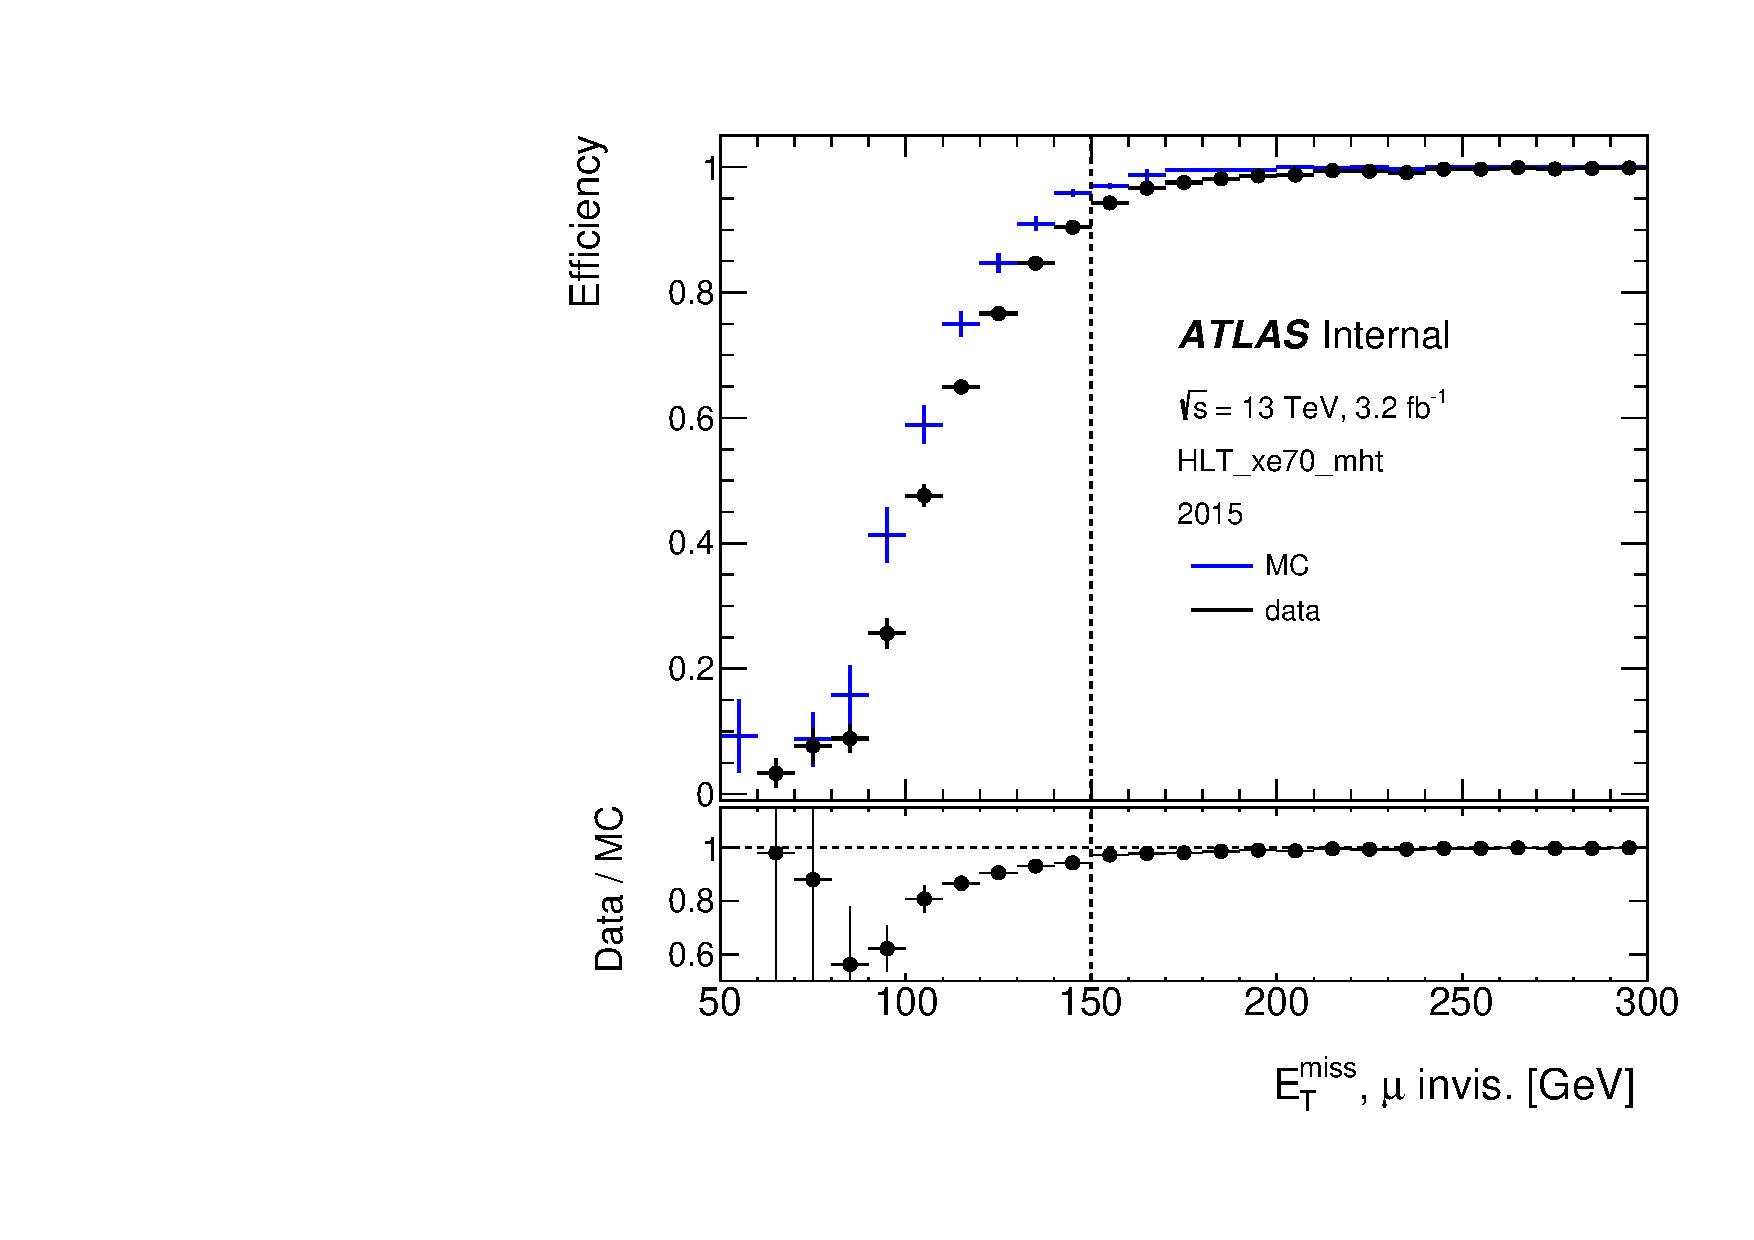
\includegraphics[width=0.45\textwidth]{fig/METTriggerCalibration/efficiecy_HLT_xe70_mht.pdf}
	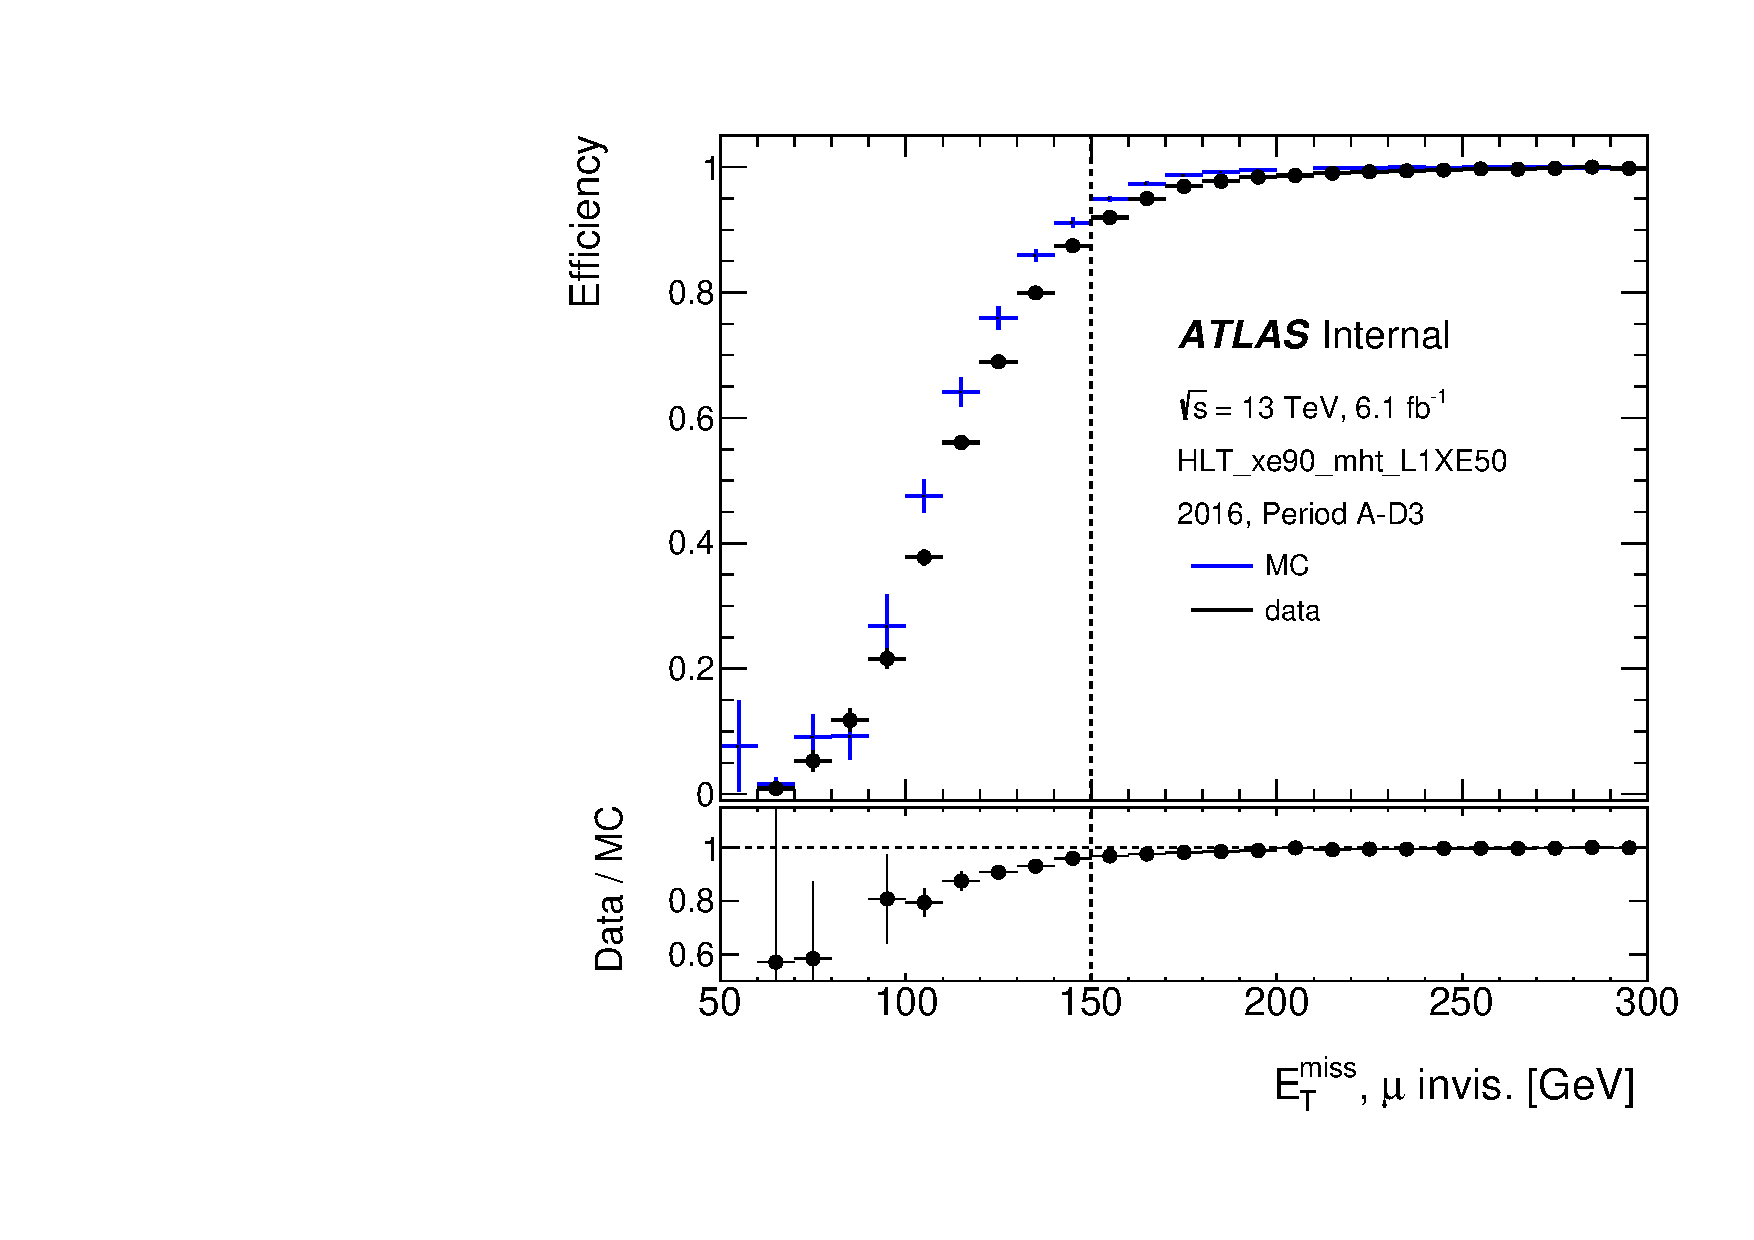
\includegraphics[width=0.45\textwidth]{fig/METTriggerCalibration/efficiecy_HLT_xe90_mht_L1XE50.pdf}
	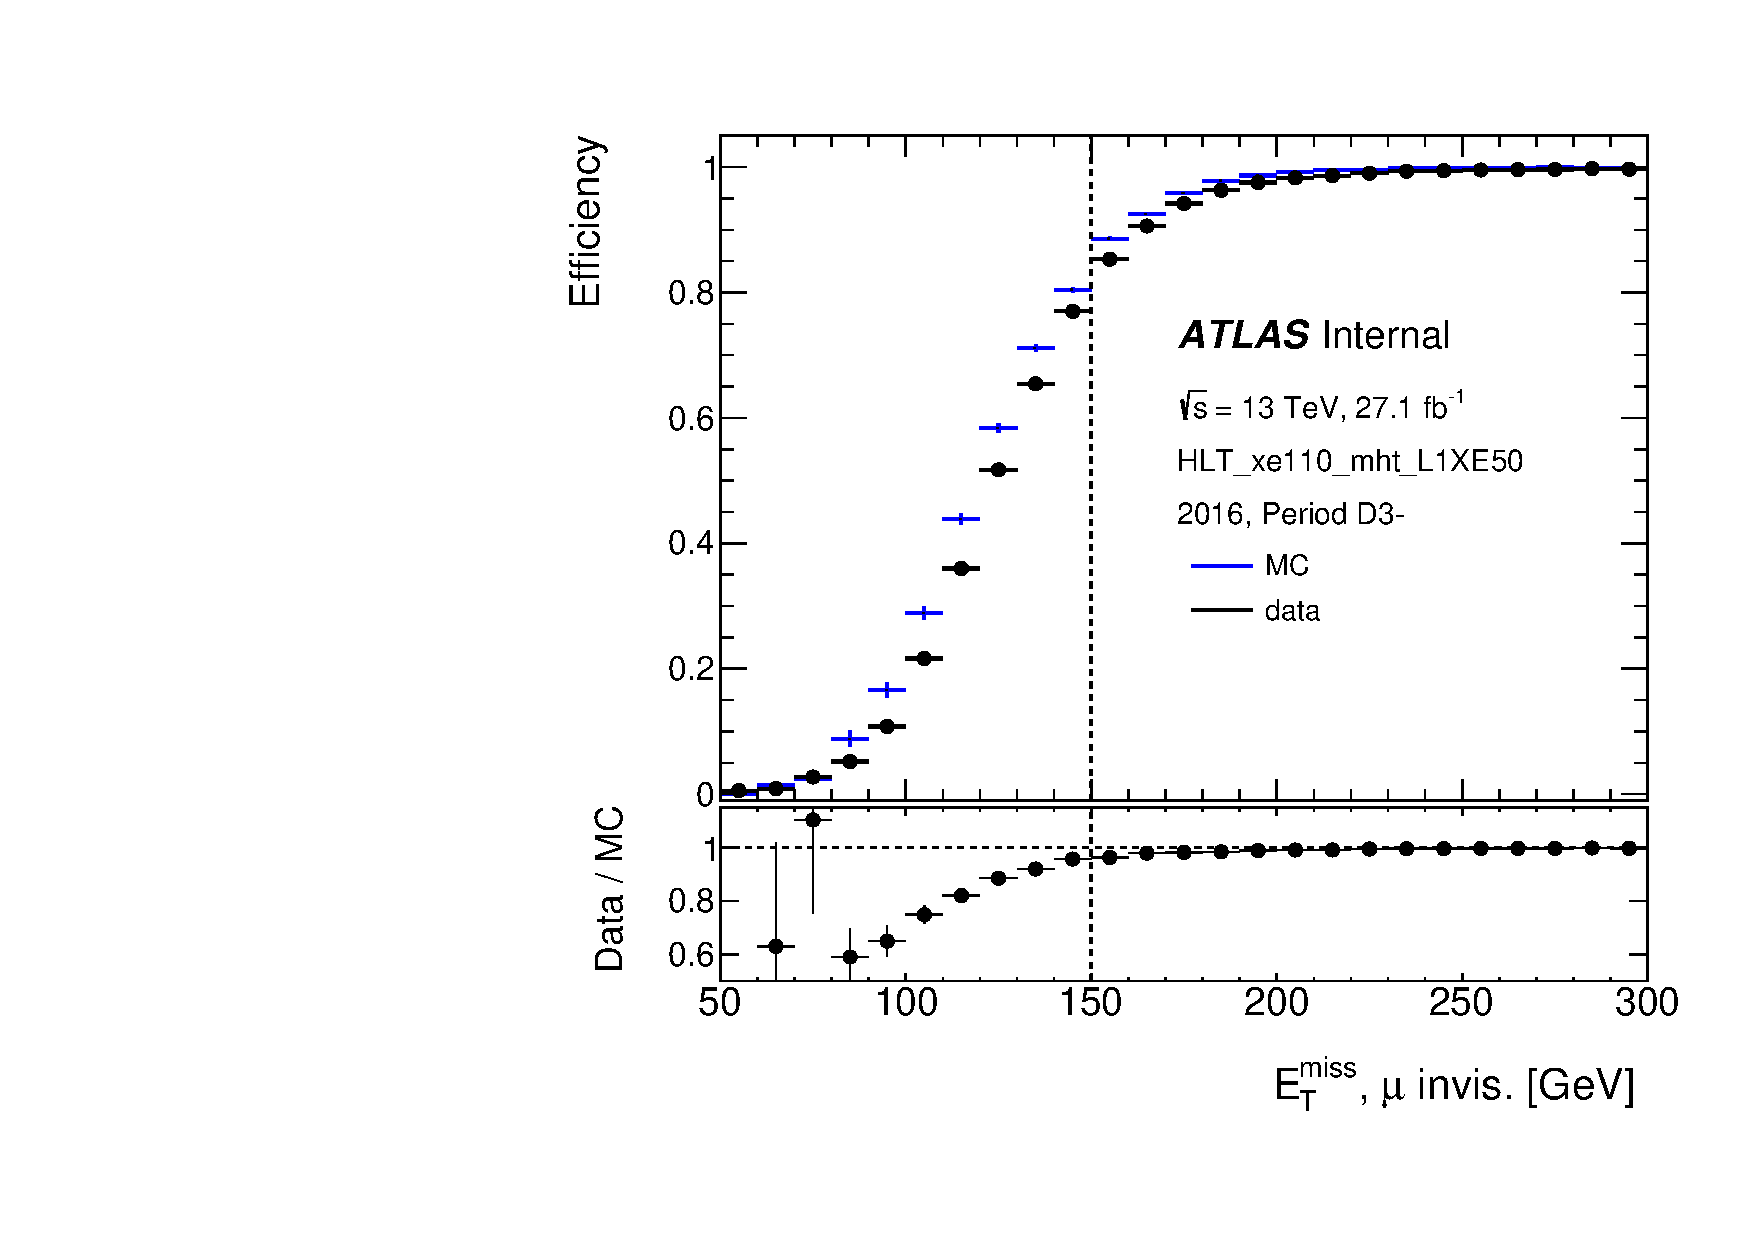
\includegraphics[width=0.45\textwidth]{fig/METTriggerCalibration/efficiecy_HLT_xe110_mht_L1XE50.pdf}
	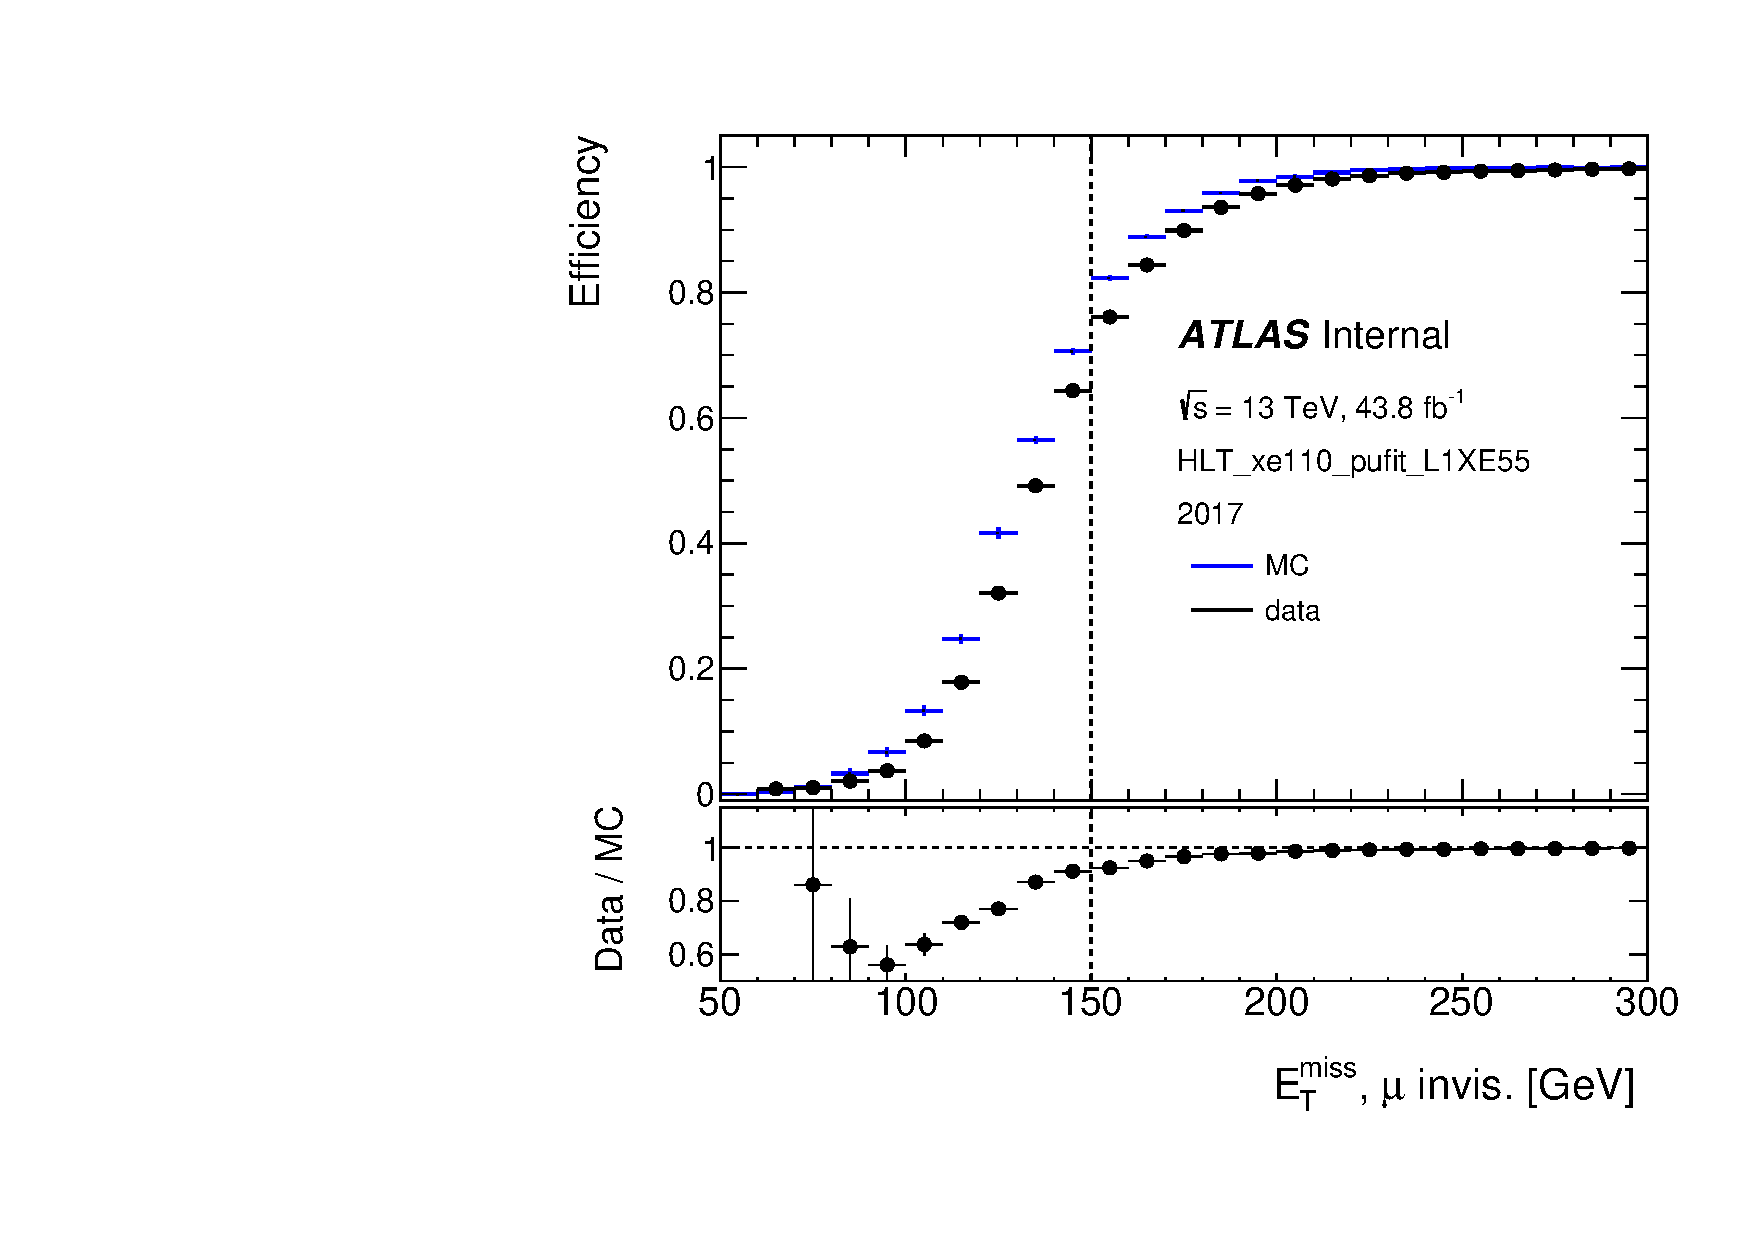
\includegraphics[width=0.45\textwidth]{fig/METTriggerCalibration/efficiecy_HLT_xe110_pufit_L1XE55.pdf}
	\caption{Measured trigger efficiencies as a function of offline \METnomu in data and MC for the \met triggers used in 2015-2018. The plots are shown for 0,1 and 2 tags together. The lower panels provide the ratio of data and MC events (the scale factor).}
	\label{fig:TrigEff}
\end{figure}
The triggers are listed in Table~\ref{tab:summary_triggers_used}. 

\begin{table}
	\scriptsize{
		\begin{center}

			\resizebox{1.\textwidth}{!}{
				\begin{tabular}{ c c c c}
					\hline
					\hline
					Period & 0 lepton & 1 lepton & 2 lepton + \met~trigger SF measurement \\
					\hline
					2015 & \textsc{HLT\_xe70\_mht} & \textsc{HLT\_xe70\_mht} & \textsc{HLT\_e24\_lhmedium\_L1EM20VH}\\
					& & & \textbf{OR} \textsc{HLT\_e120\_lhloose}  \\ 
					& & & \textbf{OR} \textsc{HLT\_mu20\_iloose\_L1MU15} \\
					& & & \textbf{OR} \textsc{HLT\_mu50} \\
					\hline
					2016 & \textsc{HLT\_xe90\_mht\_L1XE50} & \textsc{HLT\_xe90\_mht\_L1XE50} & \textsc{HLT\_e60\_lhmedium\_nod0}  \\
					(A) & & & \textbf{OR} \textsc{HLT\_e140\_lhloose\_nod0} \\ 
					& & & \textbf{OR} \textsc{HLT\_mu40} \\
					& & & \textbf{OR} \textsc{HLT\_mu50} \\
					\hline
					2016 & \textsc{HLT\_xe90\_mht\_L1XE50} & \textsc{HLT\_xe90\_mht\_L1XE50} & \\
                    (B-D3) & & & \textsc{HLT\_e60\_lhmedium\_nod0} \\
					& & & \textbf{OR} \textsc{HLT\_e140\_lhloose\_nod0} \\ 
					& & & \textbf{OR} \textsc{HLT\_mu24\_ivarmedium} \\
					& & & \textbf{OR} \textsc{HLT\_mu50} \\
					\hline
					2016 & \textsc{HLT\_xe110\_mht\_L1XE50} & \textsc{HLT\_xe110\_mht\_L1XE50} & \textsc{HLT\_e26\_lhtight\_nod0\_ivarloose} \\	
					(D4-E3)& & & \textbf{OR} \textsc{HLT\_e60\_lhmedium\_nod0} \\
					& & & \textbf{OR} \textsc{HLT\_e140\_lhloose\_nod0} \\ 
					& & & \textbf{OR} \textsc{HLT\_mu24\_ivarmedium} \\
					& & & \textbf{OR} \textsc{HLT\_mu26\_ivarmedium} \\
					& & & \textbf{OR} \textsc{HLT\_mu50} \\
					\hline
					2016 & \textsc{HLT\_xe110\_mht\_L1XE50} & \textsc{HLT\_xe110\_mht\_L1XE50} & \textsc{HLT\_e26\_lhtight\_nod0\_ivarloose}\\
                    (F1)&  & & \textbf{OR} \textsc{HLT\_e60\_lhmedium\_nod0} \\
					& & & \textbf{OR} \textsc{HLT\_e140\_lhloose\_nod0} \\ 
					& & & \textbf{OR} \textsc{HLT\_mu26\_ivarmedium} \\
					& & & \textbf{OR} \textsc{HLT\_mu50} \\
					\hline
					2016 & \textsc{HLT\_xe110\_mht\_L1XE50} & \textsc{HLT\_xe110\_mht\_L1XE50} &\textsc{HLT\_e26\_lhtight\_nod0\_ivarloose} \\
					(F2-) & & & \textbf{OR} \textsc{HLT\_e60\_lhmedium\_nod0} \\
					& & & \textbf{OR} \textsc{HLT\_e140\_lhloose\_nod0} \\ 
					& & & \textbf{OR} \textsc{HLT\_mu26\_ivarmedium} \\
					& & & \textbf{OR} \textsc{HLT\_mu50} \\
					\hline
					2017 & \textsc{HLT\_xe110\_pufit\_L1XE55} & \textsc{HLT\_xe110\_pufit\_L1XE55} &\textsc{HLT\_e60\_lhmedium\_nod0} \\
					& & & \textbf{OR} \textsc{HLT\_e140\_lhloose\_nod0} \\
					& & & \textbf{OR} \textsc{HLT\_mu26\_ivarmedium} \\
					& & & \textbf{OR} \textsc{HLT\_mu50} \\
					\hline
					2018 & \textsc{HLT\_xe110\_pufit\_70\_L1XE55} & \textsc{HLT\_xe110\_pufit\_70\_L1XE55} &  \textsc{HLT\_e60\_lhmedium\_nod0} \\
					(B-C5)& & & \textbf{OR} \textsc{HLT\_e140\_lhloose\_nod0} \\
					& & & \textbf{OR} \textsc{HLT\_mu26\_ivarmedium} \\
					& & & \textbf{OR} \textsc{HLT\_mu50} \\
					\hline
					2018 & \textsc{HLT\_xe110\_pufit\_65\_L1XE55} & \textsc{HLT\_xe110\_pufit\_65\_L1XE55} &\textsc{HLT\_e60\_lhmedium\_nod0} \\
					(C5-) & & & \textbf{OR} \textsc{HLT\_e140\_lhloose\_nod0} \\
					& & & \textbf{OR} \textsc{HLT\_mu26\_ivarmedium} \\
					& & & \textbf{OR} \textsc{HLT\_mu50} \\    		
					\hline
					\hline
				\end{tabular}}
			\end{center}
		}
		\caption{\met~and single-lepton triggers used in the analysis.}
		\label{tab:summary_triggers_used}
\end{table}
	
\section{MC samples}
\label{ch:data-mc-samples}


